%!TEX root = main.tex

\chapter{Marco Teórico}
\label{sec:introduction}

\begin{chapquote}{Carl Friedrich Gauss}
	«No es el conocimiento, sino el acto de aprender, no la posesión sino el acto de llegar, lo que otorga el mayor disfrute.»
\end{chapquote}

\comment{parrafo: resumen de todo el capitulo, si es necesario otro anterior, explicar brevemente el porque de este capitulo, asi como que contiene}



\comment{introducir un poco mas}
Los procesos gaussianos (GP por sus siglas en inglés) cumplen con la propiedad que sus distribuciones de probabilidades conjunta, marginal y condicional se pueden escribir de forma explícitas, permitiendo utilizar los GP para modelar funciones de forma no paramétricas y realizar las tareas de suavizado, interpolación y predicción en términos probabilísticos. Dichas técnicas son muy utilizada en aprendizaje de máquinas. En este libro nos concentraremos en la definición formal, propiedades, tipos y diferentes arquitecturas de los GP. Para introducir los GP es necesario presentar los conceptos básicos necesarios para poder definirlos en términos formales, empezando por probabilidades, distribuciones y procesos estocásticos.

\section{Probabilidades}
\label{sec:probability}

Un espacio muestral \(\Omega\) es un conjunto con todos los posibles resultados para modelar un cierto experimento aleatorio. Por ejemplo, si el experimento es lanzar un dado de seis caras, entonces el espacio muestral corresponde a todos los posibles resultados del dado, es decir \(\Omega = \{1, 2, 3, 4, 5, 6\}\).

Un conjunto de resultados del espacio muestral \(E \subseteq \Omega\) se denomina evento, y una \(\sigma\)-álgebra \(\calB \subseteq \calP(\Omega)\) asociada a \(\Omega\) se llama espacio de sucesos o eventos medibles. Se dice que un evento \(E\) es medible si \(E \in \calB\). Se puede interpretar que un evento es un conjunto que representa una propiedad, y por lo cual una \(\sigma\)-álgebra representa el conjunto de propiedades expresables (medibles) sobre un espacio muestral. Una \(\sigma\)-álgebra \(\calB\) cumple tres propiedades, enumeradas a continuación:
\begin{enumerate}
	\item El conjunto vacío es un evento medible, es decir \(\varnothing \in \calB\).
	\item Si \(E \in \calB\) es un evento medible entonces su complemento también lo es, es decir, \(E^\mathsf{c} \in \calB\).
	\item Si \(E_1, E_2, E_3, \dotsc\) es una sucesión de eventos medibles, entonces su unión también es un evento, es decir, \(\bigcup_{i=1}^\infty E_i \in \calB\).
\end{enumerate}

Para el ejemplo anterior, la \(\sigma\)-álgebra \(\calB = \{\Omega, \varnothing, \{1, 3, 5\}, \{2, 4, 6\}\}\) codifica los eventos que, además del vacío y el conjunto muestral, permiten distinguir los pares de los impares, pero no es posible distinguir eventos tales como \emph{menor a 3} o \emph{igual a 5}, ya que \(\calB\) no contiene ningún conjunto que coincida con esa propiedad. Si se quisiera codificar los eventos \emph{menor a 3} e \emph{igual a 5}, entonces la \(\sigma\)-álgebra que contiene todos los eventos generados por complemento e uniones es la siguiente: \[\calB = \big\{\Omega, \varnothing, \{1, 2\}, \{3, 4, 5, 6\}, \{5\}, \{1, 2, 3, 4, 6\}, \{1, 2, 5\}, \{3, 4, 6\}\big\}.\]

Si se quisiera poder distinguir (i.e. medir) otros tipos de eventos adicionales, entonces es necesaria una \(\sigma\)-álgebra \(\hat{\calB}\) más \emph{grande} que \(\calB\), de modo que \(\calB \subset \hat{\calB}\). Tal \(\sigma\)-álgebra se dice \emph{más fina}. Es claro que la \(\sigma\)-álgebra \(\calB = \calP(\Omega)\), el conjunto potencia de las partes de \(\Omega\) que contiene a todos los conjuntos posibles, es la \(\sigma\)-álgebra más fina, pues todo es medible. Esto siempre es posible de aplicar en el caso en que \(\Omega\) es discreto, pero no en el caso infinito.

Finalmente, una medida o ley de probabilidad \(\prob\) en el espacio muestral \(\Omega\) es una función que a cada evento \(E\) de la \(\sigma\)-álgebra \(\calB\) le asigna un valor entre \(0\) y \(1\) (su probabilidad) y cumple con las siguientes propiedades:
\begin{enumerate}
	\item Para todo \(E \in \calB\) se tiene que \(0 \leq \prob(E) \leq 1\).
	\item \(\prob(\varnothing) = 0\) y \(\prob(\Omega) = 1\).
	\item Si \(E_1, E_2, E_3, \dotsc\) es una sucesión de eventos disjuntos, es decir, \(E_i \cap E_j = \varnothing\) para \(i \neq j\), entonces \(\prob(\bigcup_{i=1}^\infty E_i) = \sum_{i=1}^\infty \prob(E_i)\).
\end{enumerate}

Lo que codifican las 3 propiedades anteriores es que una medida de probabilidad es consistente con las operaciones de conjuntos, es decir, mide bien los eventos medibles. Un espacio muestral \(\Omega\) dotado de una \(\sigma\)-álgebra \(\calB \subseteq \calP(\Omega)\) y una medida o ley de probabilidades \(\prob : \calB \to [0, 1]\) se llama espacio de probabilidades.

De las propiedades anteriores se derivan otras más, tales como que la probabilidad del evento complemento se puede expresar como el «complemento» de la probabilidad del evento, es decir \(\prob(A^\mathsf{c}) = 1 - \prob(A)\). Una medida de probabilidad es una forma de medir los eventos de una \(\sigma\)-álgebra de forma consistente. Para el ejemplo del dado, suponiendo que este es equiprobable, la medida de probabilidad se define completamente por \(\prob(\{1, 3, 5\}) = \frac{1}{2}\), que asigna la misma probabilidad a los pares e impares. Sin embargo, dependiendo de que tan equilibrado sea el dado, existen infinitas medidas de probabilidad que asigna \(\prob(\{1, 3, 5\}) = p\) y \(\prob(\{2, 4, 6\}) = 1 - p\), con \(p \in [0, 1]\). Este experimento es muy similar a lanzar una moneda.

\comment{parrafo: aterrizada del tema, pequeño resumen y encadenar al siguiente tema}

\subsection{Independencia y Condicionalidad}

\comment{parrafo: continuar con encadenamiento anterior, establecer brevemente que sera esta seccion}

Sea \((\Omega, \calB, \prob)\) un espacio de probabilidades. Se puede interpretar el concepto de independencia entre dos (o más) eventos medibles como que el resultado de un evento no afecta al otro y viceversa. Un ejemplo de eventos independientes es el lanzamiento de dos monedas, ya que el resultado de una moneda no afecta el resultado de la otra moneda. La definición formal de independencia es que la probabilidad de que ambos eventos sucedan a la vez es igual a la multiplicación de las probabilidades de ambos eventos.

\begin{definition}
	Sean \(A, B \in \calB\) dos eventos medibles. \(A\) se dice independiente de \(B\), denotando que \(A \perp B\), si y solo si \(\prob (A, B) = \prob (A \cap B) = \prob (A) \prob (B)\).
\end{definition}

Formalizando el ejemplo, tenemos que el espacio muestral son los cuatro posibles resultados de lanzar dos monedas es \(\Omega = \{(\mathrm{c}, \mathrm{c}), (\mathrm{c}, \mathrm{s}), (\mathrm{s}, \mathrm{c}), (\mathrm{s}, \mathrm{s})\}\), donde «c» y «s» denotan que el resultado sea cara o sello, respectivamente. Como este caso es discreto, se puede usar la \(\sigma\)-álgebra potencia \(\calB = \calP(\Omega)\), y la medida de probabilidades equiprobable, es decir, \(\prob(\{(\mathrm{e}_1, \mathrm{e}_2)\}) = \frac{1}{4}\), para dos resultados cualquiera. Calculando para \(A = \{(\mathrm{e}_1, \mathrm{c}), (\mathrm{e}_1, \mathrm{s})\}, B = \{(\mathrm{c}, \mathrm{e}_2), (\mathrm{s}, \mathrm{e}_2)\}\) con \(\mathrm{e}_1, \mathrm{e}_2 \in \{\mathrm{c}, \mathrm{s}\}\), se tiene que:
\begin{equation*}
	\prob (A, B) = \prob(\{(\mathrm{e}_1, \mathrm{e}_2)\}) = \frac{1}{4} = \frac{1}{2} \cdot \frac{1}{2} = \prob(\{(\mathrm{e}_1, \mathrm{c}),(\mathrm{e}_1, \mathrm{s})\}) \prob(\{(\mathrm{c}, \mathrm{e}_2), (\mathrm{s}, \mathrm{e}_2)\}) = \prob(A) \prob(B).
\end{equation*}

Otro concepto importante es el de probabilidad condicional entre dos eventos medibles.
\begin{definition}
	Sean \(A, B \in \calB\) dos eventos medibles tales que \(\prob(B) > 0\). La probabilidad condicional de \(A\) dado \(B\) se define como \(\prob(A \mid B) \coloneqq \frac{\prob(A, B)}{\prob(B)}\).
\end{definition}

La forma de interpretar la probabilidad condicional del evento \(A\) dado el evento \(B\) es suponer cierta la propiedad que representa a \(B\), y se quiere calcular la medida de probabilidad de \(A\) bajo ese supuesto.

Por ejemplo, considere que tiene un libro rojo para niños, un libro rojo para adultos, dos libros azules para niños y tres libros azules para adultos. En este caso se puede ver que los eventos «libro azul» y «libro para niños» no son independientes, ya que
\[\prob(\textrm{niño}, \mathrm{azul}) = \frac{2}{7} \neq \frac{3}{7} \cdot \frac{5}{7} = \prob(\textrm{niño}) \prob(\textrm{azul}).\]
Si se saca completamente al azar un libro, surge la pregunta: ¿cuál es la probabilidad de sacar un libro de niño, dado que se sacó un libro azul? La respuesta es
\[\prob(\textrm{niño} \mid \textrm{azul}) = \frac{\prob(\textrm{niño}, \textrm{azul})}{\prob(\textrm{azul})} = \frac{2}{5}.\]

Con estas primeras definiciones, se pueden deducir simples pero poderosas propiedades que permitirán inferir probabilidades de eventos desconocidos (abajo denotados \(A\)) a partir de datos (abajo denotados \(E\)):

\begin{theorem}[Teorema de Bayes]
	La probabilidad condicional de un evento \(A\) dado un evento \(E\) puede escribirse como
	\[\prob(A \mid E) = \frac{\prob(E \mid A) \prob(A)}{\prob(E)},\]
	donde \(\prob(A \mid E)\) se llama la distribución \emph{a posteriori} de \(A\) dado \(E\), \(\prob(E \mid A)\) se conoce como la verosimilitud de los datos, \(\prob(A)\) es la probabilidad \emph{a priori} de \(A\) y \(\prob(E)\) es la probabilidad de los datos.
\end{theorem}

La demostración del teorema de Bayes es bastante directa, ya que basta con expandir la definición de probabilidad condicional y simplificar. Sin embargo, a lo largo de este libro se verá que esta propiedad tiene una implicancia fundamental en el paradigma bayesiano, el cual permite aplicar el teorema de Bayes a través de diferentes niveles conceptuales.

Existe una relación entre independencia y probabilidad condicional, dada por la siguiente propiedad:
\begin{proposition}
	Dos eventos \(A\) y \(B\) son independientes si y solo si la distribución \emph{a priori} y \emph{a posteriori} coinciden, es decir, \(A \perp B \iff \prob(A \mid B) = \prob(A)\).
\end{proposition}
Lo anterior se puede interpretar como que si dos eventos son independientes entonces un evento no agrega información al otro evento, y viceversa. Mezclando los conceptos de independencia y condicionalidad, se puede definir la independencia condicional de la siguiente forma.

\begin{definition}
	\(A\) se dice independiente de \(B\) dado \(E\), denotado \(A \perp B \mid E\) si y solo si \(\prob(A, B \mid E) = \prob(A \mid E) \prob(B \mid E)\). Esta propiedad se llama independencia condicional.
\end{definition}
Esta definición es bastante poderosa, pues si se considera \(E = \Omega\) se obtiene la definición de independencia vista inicialmente. Se puede interpretar que \(E\) representa la información (o datos) que se tiene en cierto momento, y esta información puede hacer que dos eventos que no son independientes se conviertan en independientes de forma condicional a \(E\). De forma similar al caso estándar, se puede enunciar la siguiente proposición:
\begin{proposition}
	Dos eventos \(A\) e \(B\) son independientes condicionados al evento \(E\) si y solo si la probabilidad de \(A\) dado \(B, E\) coincide con la probabilidad de \(A\) dado solo \(E\), es decir, \(A \perp B \mid E \iff \prob (A \mid B, E) = \prob (A \mid E)\).
\end{proposition}

Las siguientes proposiciones son reglas que permiten calcular probabilidades bajo el paradigma de «divide y vencerás», descomponiendo el cálculo deseado en otros más simples.
\begin{proposition}[Regla de Marginalización]
	Sea \(\{E_i\}_{i \in \naturals}\) una partición de \(\Omega\) (conjuntos disjuntos tales que \(\bigcup\limits_{i\in \naturals} E_i = \Omega\)). Entonces la probabilidad de \(A\) se puede expresar como:
	\[\prob(A) = \sum_{i \in \naturals} \prob(A \mid E_i) \prob(E_i).\]
\end{proposition}

\begin{proposition}[Regla de la Cadena]
	Sean \(E_1, \dotsc, E_N\) eventos medibles. Entonces su probabilidad conjunta puede escribirse como
	\[\prob (E_1, \dotsc, E_N) = \prob(E_1) \prod_{i=2}^N \prob (E_i \mid E_1, \dotsc, E_{i-1}).\]
\end{proposition}

\subsection{Distribuciones de Probabilidades}
\label{sec:distributions}
Ahora que los conceptos de eventos y medida de un espacio de probabilidades están definidos, se puede estudiar cómo se comportan las funciones que van desde dicho espacio al conjunto de los reales. Se introducen a continuación los conceptos de las funciones conocidas como variables aleatorias.

\begin{definition}
	Una variable aleatoria \(X\) es una función medible de \(\Omega\) a valores en \(\reals\), es decir, \(X(\omega) \in \reals\) con \(\omega \in \Omega\). Se dice que \(X\) es un vector aleatorio si es una función medible de \(\Omega\) a valores en \(\reals^n\).
\end{definition}

Que \(X\) sea medible significa que, dado que \(\reals\) está dotado de una \(\sigma\)-álgebra (normalmente la \(\sigma\)-álgebra de Borel o de Lebesgue), la preimagen \(X^{-1}(E)\) es medible en \(\Omega\) para todo conjunto \(E\) medible en \(\reals\).

Una variable aleatoria tiene múltiples propiedades, pero existen dos valores muy utilizados en la literatura, que corresponden a una medida central y a una medida de dispersión, llamadas esperanza (o media) y varianza respectivamente.
\begin{definition}
	Dada una variable aleatoria \(X\), se definen su esperanza y varianza como
	\begin{align*}
		\mu_X		&= \mean(X) = \int_\Omega X(\omega) \dd{\prob(\omega)},\\
		\sigma_X^2	&= \variance(X) = \int_\Omega (X(\omega) - \mu_X)^2 \dd{\prob(\omega)}.
	\end{align*}
\end{definition}

Una propiedad muy deseada de una variable aleatoria \(X\) es contar con una función \(F\), llamada función de distribución de probabilidades, que permita calcular la probabilidad de eventos de la forma \(E = \{\omega \in \Omega : X(\omega) \leq c\}\) evaluando \(F(c)\).

\begin{definition}
	Dada una variable aleatoria \(X\) a valores reales, se dice que \(X\) sigue una distribución de probabilidades si existe una función \(F\) que cumple:
	\begin{enumerate}
		\item \(F\) es no decreciente,
		\item \(F\) es continua por la derecha,
		\item \(F : \reals \to [0,1]\),
		\item \(F(x) \to 0\) cuando \(x \to -\infty\), y \(F(x) \to 1\) cuando \(x \to \infty\),
	\end{enumerate}
	y tal que para todo \(c \in \reals\), \(\prob(\{\omega \in \Omega : X(\omega) \leq c\}) = F(c)\). Se dice además que \(X\) tiene una función de densidad \(f\) (también denotada como \(p\)) si se cumple que
	\begin{equation*}
		F(c) = \int_{-\infty}^c f(x) \dd{x} = \int\limits_{\{\omega \in \Omega : X(\omega) \leq c\}} \dd{\prob(\omega)}.
	\end{equation*}
\end{definition}

La imagen de la variable aleatoria \(X(\Omega) \subseteq \reals\) se conoce como el soporte de la distribución \(F\). Si el soporte de \(F\) es numerable entonces se dirá que la variable aleatoria sigue una distribución discreta, en caso contrario se dice que sigue una distribución continua. En el caso discreto las integrales se reemplazan por sumatorias, ya que la función de densidad corresponde a una función de masa puntual correspondiente a una suma de distribuciones delta de Dirac \(\delta_i\):
\begin{align*}
	F(c) &= \sum_{i\leq c} p_i,		& f(x) &= \sum_{i \in \naturals} p_i \delta_i(x).
\end{align*}

Si la función de densidad \(f(x)\) de una variable aleatoria \(X\) es conocida, entonces se pueden calcular las probabilidades de eventos asociados a dicha variable sin la necesidad de conocer directamente \(\prob\). En particular es posible calcular su esperanza y varianza en función de \(f\).

\begin{proposition}
	Dada una variable aleatoria \(X\) con densidad de probabilidad \(f\), se tiene que su esperanza y ¸varianza son
	\begin{align*}
		\mu_X		&= \mean(X) = \int_{\reals} x f(x) \dd{x}, \\
		\sigma_X^2	&= \variance(X) = \int_{\reals} (x - \mu_X)^2 f(x) \dd{x}.
	\end{align*}
\end{proposition}

Finalmente, el concepto de independencia entre variables aleatorias \(X\), \(Y\) con distribuciones de probabilidad \(F_X\), \(F_Y\) es equivalente a que la distribución conjunta, asociada a la variable aleatoria \((X, Y)\), exista y que esta sea la multiplicación de las funciones de distribución, es decir, si \(X, Y\) son dos variables aleatorias con distribuciones \(F_X, F_Y\) respectivamente, entonces la función de distribución conjunta existe y está dada por \(F_{X, Y}(x, y) = F_X(x) F_Y(y)\).

\subsection{Distribuciones Discretas}

En esta sección se presentan las distribuciones discretas más utilizadas. Para cada una de ellas se lista una breve descripción, los parámetros necesarios para definirla, su conjunto soporte, su función de densidad de probabilidad \(f\), su media \(\mu_X\) y su varianza \(\sigma^2_X\). En muchas de ellas se usa un parámetro \(p \in [0, 1]\) y se denota por \(q = 1 - p\).

\begin{enumerate}
	\item La distribución \textbf{degenerada} es aquella que concentra toda la probabilidad en solo un punto. Se define con solo un parámetro \(c \in \reals\). Su conjunto soporte es \(\{c\}\), y la densidad es
	\[ f(k) = \begin{dcases*}
		1,	& si \(k = c\),\\
		0,	& en otro caso.
	\end{dcases*} \]
	Su media es \(\mu_X = c\) y su varianza es \(\sigma^2_X = 0\).
	\item La distribución \textbf{uniforme} es aquella que le asigna la misma probabilidad a cada punto en un conjunto. Sus parámetros son \(c_1, \dotsc, c_n \in \reals\). Su conjunto soporte es \(\{c_1, \dotsc, c_n\}\) y la densidad es \(f(c_i) = 1 / n\). Su media y su varianza son
	\begin{align*}
		\mu_X		&= \frac{1}{n} \sum_{i=1}^n c_{i},	& \sigma^2_X	&= \frac{1}{n} \sum_{i=1}^n (c_i - \mu)^{2}.
	\end{align*}
	\item La distribución \textbf{Bernoulli} modela un experimento aleatorio con dos resultados posibles. Su parámetro es \(p \in [0, 1]\), la probabilidad de éxito. Su conjunto soporte es \(\{0, 1\}\) y su densidad es
	\[f(k) = \begin{dcases*}
		p,		& si \(k = 1\),\\
		1-p,	& si \(k = 0\).
	\end{dcases*}\]
	Su media es \(\mu_X = p\) y su varianza es \(\sigma^2_X = p (1-p)\).
	\item La distribución \textbf{binomial} modela el número de éxitos obtenidos en una serie de experimentos tipo Bernoulli. Sus parámetros son \(n \in \naturals\), el número de intentos; y \(p \in [0, 1]\), la probabilidad de éxito. Su soporte es \(\{0, \dotsc, n\}\), y su densidad es
	\[f(k) = \binom{n}{k} p^k q^{n-k}.\]
	Su media es \(\mu_X = np\) y su varianza es \(\sigma^2_X = npq\).
	\item La distribución \textbf{geométrica} modela el número de fracasos hasta obtener un éxito. Su parámetro es \(p \in [0, 1]\), la probabilidad de éxito. Su soporte es \(\naturals\), y su densidad es \(f(k) = q^{k} p\). Su media es \(\mu_X = q / p\) y su varianza es \(\sigma^2_X = q / p^2\).
	\item La distribución \textbf{binomial negativa} modela el número de fracasos hasta obtener un número fijo de éxitos. Sus parámetros son \(r \in \naturals\), el número de éxitos; y \(p \in [0, 1]\), la probabilidad de éxito. Su soporte es \(\naturals\), y su densidad es
	\[f(k) = \binom{k + r - 1}{k} q^k p^{r}.\]
	Su media es \(\mu_X = rq / p\) y su varianza es \(\sigma^2_X = rq / p^2\).
	\item La distribución de \textbf{Poisson} modela el número de veces que ocurre un suceso en un cierto intervalo, suponiendo que ocurren a cierta tasa e independientes entre sí. Su parámetro es \(\lambda > 0\), la tasa de ocurrencia. Su soporte es \(\naturals\), y su densidad es
	\[f(k) = \frac{e^{-\lambda} \lambda^k}{k!}.\]
	Su media es \(\mu_X = \lambda\) y su varianza es \(\sigma^2_X = \lambda\).
	\item La distribución \textbf{hipergeométrica} modela el número de éxitos en \(n\) intentos, pero sin reemplazo, en donde el número de la población \(N\) y el número de la población que se considera «exitosa» \(K\) están fijos. Sus parámetro son \(N \in \naturals\), el tamaño de la población; \(K \in \{0, \dotsc, N\}\), el tamaño de la población que se considera «exitosa»; y \(n \in \{0, \dotsc, N\}\), el número de intentos. Su soporte es el conjunto \(\{k \mid \max\{0, n+K-N\} \leq k \leq \min\{K, n\}\}\), y su densidad es
	\[f(k) = \frac{\binom{K}{k} \binom{N-K}{n-k}}{\binom{N}{n}}.\]
	Su media y su varianza son
	\begin{align*}
		\mu_X		&= n\frac{K}{N},	& \sigma^2_X	&= n\frac{K}{N} \frac{N-K}{N} \frac{N-n}{N-1}.
	\end{align*}
\end{enumerate}

\subsection{Distribuciones Continuas}

Así como con las distribuciones discretas, en esta sección se presentan las continuas discretas más utilizadas, con una breve descripción, los parámetros necesarios para definirla, su conjunto soporte, su función de densidad de probabilidad \(f\), su media \(\mu_X\) y su varianza \(\sigma^2_X\).

\begin{enumerate}
	\item La distribución \textbf{uniforme}, así como su par discreto, le asigna la misma probabilidad a un conjunto de puntos, pero esta vez el conjunto es un intervalo. Sus parámetros son \(a, b \in \reals\) con \(a < b\). Su soporte es \([a, b]\), y su densidad es \(f(x) = 1 / (b-a)\). Su media es \(\mu_X = (a+b) / 2\) y su varianza es \(\sigma^2_X = (b-a)^2 / 12\).
	\item La distribución \textbf{normal} o \textbf{gaussiana} modela una suma de un gran número de elementos independientes, y muchas veces se usa para modelar eventos que se sabe son aleatorios, pero cuya distribución es desconocida. Sus parámetros son \(\mu \in \reals\), la media; y \(\sigma^2 > 0\), la varianza. Su soporte es \(\reals\), y su densidad es
	\[f(x) = \frac{1}{\sigma \sqrt{2\pi}} \exp\biggl(-\frac{(x - \mu)^2}{2 \sigma^2}\biggr).\]
	Su media y su varianza son, valga la redundancia, \(\mu_X = \mu\) y \(\sigma^2_X = \sigma^2\).
	\item La distribución \textbf{log-normal}, similar a la normal, modela un producto de un gran número de elementos independientes. Sus parámetros son \(\mu \in \reals\), la media del logaritmo de la variable aleatoria; y \(\sigma^2 > 0\), la varianza del logaritmo de la variable aleatoria. Su soporte es \(\reals\), y su densidad es
	\[f(x) = \frac{1}{x \sigma \sqrt{2\pi}} \exp\biggl(-\frac{(\ln(x) - \mu)^2}{2 \sigma^2}\biggr).\]
	Su media y su varianza son
	\begin{align*}
		\mu_X	&= e^{\mu + \frac{\sigma^2}{2}},	& \sigma^2_X &= (e^{\sigma^2}-1)(e^{2\mu + \sigma^2}).
	\end{align*}
	\item La distribución \textbf{logística} modela procesos de crecimiento con estados de saturación. Sus parámetros son \(\mu \in \reals\), la locación; y \(s > 0\), la escala. Su soporte es \(\reals\), y su densidad es
	\[f(x) = \frac{e^{-\frac{x-\mu}{s}}}{s(1+e^{-\frac{x-\mu}{s}})^2}.\]
	Su media es \(\mu_X = \mu\) y su varianza es \(\sigma_X^2 = s^2 \pi^2 / 3\).
	\item La distribución \textbf{exponencial} modela el tiempo que ocurre entre dos sucesos consecutivos que ocurren a tasa constante (cf. distribución de Poisson). Su parámetro es \(\lambda > 0\), la tasa. Su soporte es \([0, \infty)\), y su densidad es \(f(x) = \lambda e^{-\lambda x}\). Su media es \(\mu_X = \lambda^{-1}\) y su varianza es \(\sigma_X^2 = \lambda^{-2}\).
	\item La distribución \textbf{gamma} modela el tiempo de espera hasta que un suceso ocurra un cierto número de veces. Sus parámetros son \(k > 0\), la forma (o número de veces que el suceso debe ocurrir); y \(\lambda > 0\), la tasa. Su soporte es \((0, \infty)\), y su densidad es
	\[f(x) = \lambda^k e^{-\lambda x}\frac{x^{k-1}}{\Gamma(k)}.\]
	Su media es \(\mu_X = k / \lambda\) y su varianza es \(\sigma_X^2 = k / \lambda^2\).
	\item La distribución \textbf{beta} se usa para modelar el comportamiento aleatorio de porcentajes y proporciones. Sus parámetros son \(\alpha > 0\) y \(\beta > 0\), ambos llamados «de forma». Su soporte es \([0, 1]\), y su densidad es
	\[f(x) = \frac{\Gamma(\alpha + \beta)}{\Gamma(\alpha) \Gamma(\beta)} x^{\alpha-1}(1-x)^{\beta-1}.\]
	Su media y su varianza son
	\begin{align*}
		\mu_X	&= \frac{\alpha}{\alpha + \beta},	& \sigma^2_X	&= \frac{\alpha\beta}{(\alpha+\beta+1)(\alpha + \beta)^2}.
	\end{align*}
	\item La distribución \(\boldsymbol{\chi}^2\) \textbf{de Pearson} modela pruebas de independencia, homogeneidad, bondad de ajuste, y la construcción de intervalos de confianza. Su parámetro es \(n \in \naturals_{\geq 0}\), los grados de libertad. Su soporte es \((0, \infty)\) si \(n = 1\), y \([0, \infty)\) en otro caso, y su densidad es
	\[f(x) = \frac{e^{-\frac{x}{2}} x^{\frac{n}{2}-1}}{2^{\frac{n}{2}} \Gamma(\frac{n}{2})}.\]
	Su media es \(\mu_X = n\) y su varianza es \(\sigma^2_X = 2n\).
	\item La distribución \(\bft\) \textbf{de Student} se usa para estimar la media de muestras que son normalmente distribuidas, pero son pequeñas y la varianza es desconocida. Su parámetro es \(\nu > 0\), los grados de libertad (parámetro real, cf. distribución \(\chi^2\) de Pearson, donde los grados de libertad son enteros). Su soporte es \(\reals\), y su densidad es
	\[f(x) = \frac{\Gamma(\frac{\nu+1}{2}) (1 + \frac{x^2}{\nu})^{-\frac{\nu + 1}{2}}}{\sqrt{\nu \pi} \Gamma(\frac{\nu}{2})}.\]
	Su media es \(\mu_X = 0\) y su varianza es
	\[\sigma^2_X = \begin{dcases*}
		\frac{\nu}{\nu - 2},	& si \(\nu > 2\),\\
		\infty,					& si \(1 < \nu \leq 2\),\\
		\text{indefinida},		& en otro caso.
	\end{dcases*}\]
	\item La distribución \textbf{F de Fisher-Snedecor} se usa en pruebas de ANOVA para comparar varianzas entre poblaciones, y como la distribución de la hipótesis nula. Sus parámetros son \(n > 0\) y \(m > 0\), los grados de libertad (si bien usualmente estos grados son naturales, la distribución está bien definida para grados de libertad reales). Su soporte es \((0, \infty)\) si \(m = 1\), y \([0, \infty)\) en otro caso, y su densidad es
	\[f(x) = \frac{\sqrt{\frac{(mx)^m n^n}{(mx+n)^{n+m}}}}{x B(\frac{m}{2}, \frac{n}{2})},\]
	donde \(B\) es la función beta. Su media es \(\mu_X = n / (n - 2)\) solo cuando \(n > 2\) y su varianza es
	\[\sigma^2_X = \frac{2n^2 (n+m-2)}{m(n-2) (n-4)},\]
	solo cuando \(n > 4\). En otro caso, están indefinidas.
	\item La distribución de \textbf{Cauchy} modela la distancia horizontal de un segmento con un ángulo aleatorio, así como la razón entre dos variables aleatorias independientes normales de media cero. Sus parámetros son \(x_0 \in \reals\), la locación; y \(\gamma > 0\), la escala. Su soporte es \(\reals\), y su densidad es
	\[f(x) = \frac{1}{\pi} \left[\frac{\gamma}{(x - x_0)^2 + \gamma^2} \right].\]
	Tanto su media como su varianzas están indefinidas.
	\item La distribución de \textbf{Weibull} modela la vida útil de un sistema donde la tasa de error cambia con el tiempo, y es muy usada en teoría de valores extremos. Sus parámetros son \(\lambda > 0\), la escala; y \(k > 0\), la forma. Su soporte es \([0, \infty)\), y su densidad es
	\[f(x) = \frac{k}{\lambda}\Bigl(\frac{x}{\lambda}\Bigr)^{k-1} \exp(-\Bigl(\frac{x}{\lambda}\Bigr)^k).\]
	Su media y su varianza son
	\begin{align*}
		\mu_X	&= \lambda \Gamma\biggl(\frac{k+1}{k}\biggr),	& \sigma^2_X	& = \lambda^2 \Gamma\biggl(\frac{k+2}{k}\biggr) - \mu^2.
	\end{align*}
	\item La distribución de \textbf{Laplace} se usa en reconocimiento de audio para modelar coeficientes de la transformada de Fourier discreta, así como en movimientos brownianos exponenciales. Sus parámetros son \(\mu \in \reals\), la locación; y \(b > 0\), la escala. Su soporte es \(\reals\), y su densidad es
	\[f(x) = \frac{1}{2b} \exp(-\frac{\lvert x - \mu \rvert}{b}).\]
	Su media es \(\mu_X = \mu\) y su varianza es \(\sigma_X^2 = 2b^2\).
	\item La distribución de \textbf{Pareto} modela la distribución de la riqueza en una sociedad y procesos que siguen la ley de Zipf. Sus parámetros son \(x_m > 0\), la escala; y \(\alpha > 0\), la forma. Su soporte es \([x_m, \infty)\), y su densidad es \(f(x) = \alpha x_m^\alpha / x^{\alpha + 1}\). Su media y su varianza son
	\begin{align*}
		\mu_X	&= \frac{x_m}{\alpha-1},	& \sigma^2_X	&= \frac{x_m^2 \alpha}{(\alpha-1)^2 (\alpha-2)}.
	\end{align*}
	\item La distribución de \textbf{Gumbel} modela la distribución del máximo o mínimo para calcular valores extremos. Sus parámetros son \(\mu \in \reals\), la locación; y \(\beta > 0\), la escala. Su soporte es \(\reals\), y su densidad es
	\[f(x) = \frac{1}{\beta} \exp(-\frac{x-\mu}{\beta} - \exp(-\frac{x-\mu}{\beta})).\]
	Su media es \(\mu_X = \mu + \beta \gamma\), con \(\gamma\) la constante de Euler--Mascheroni, y su varianza es \(\sigma_X^2 = \pi^2 \beta^2 / 6\).
	\item La distribución \textbf{triangular} se usa para describir a una población cuando hay datos limitados y cuando se sabe que hay una relación entre variables, pero los datos son escasos. Sus parámetros son \(a \in \reals\), el límite inferior; \(b > a\), el límite superior; y \(c \in [a, b]\), la moda. Su soporte es \([a, b]\), y su densidad es
	\[f(x) = \begin{dcases*}
		\frac{2(x-a)}{(b-a)(c-a)},	& si \(x \in [a, c)\),\\
		\frac{2}{b-a},				& si \(x = c\),\\
		\frac{2(b-x)}{(b-a)(b-c)},	& si \(x \in (c, b]\).
	\end{dcases*}\]
	Su media es \(\mu_X = (a+b+c) / 3\) y su varianza es
	\[\sigma^2_X = \frac{a^2 + b^2 + c^2 - ab - ac - bc}{18}.\]
\end{enumerate}

\subsection{Distribución Gaussiana}

Para poder definir un proceso gaussiano, es necesario estudiar su elemento basal: la distribución normal o gaussiana. Valga la redundancia, su definición es la siguiente:
\begin{definition}
	Se dice que una variable aleatoria \(X\) a valores reales sigue una distribución normal de media \(\mu \in \reals\) y varianza \(\sigma^2 > 0\), denotada \(\calN \left(\mu, \sigma^2\right)\), si su función de densidad está dada por
	\[ f( x; \mu, \sigma) = \frac{1}{\sqrt{2\pi} \sigma} e^{-\frac{(x - \mu)^2}{2\sigma^2}}.\]
\end{definition}

\begin{figure}[h]
	\centering
	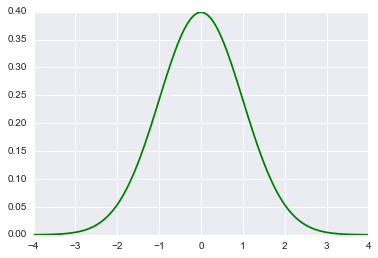
\includegraphics[scale=0.55]{normal}
\end{figure}

Como la densidad solo depende de \(\mu\) y \(\sigma^2\), conociendo estos dos valores se define por completo su función de distribución. Más aún, estos valores coinciden con la media y la varianza, por lo que la distribución normal es definida completamente con sus dos primeros momentos:
\begin{align*}
	\mean(X)		&= \mu,\\
	\variance(X)	&= \sigma^2.
\end{align*}
Para ayudar a entender por qué esta distribución es tan importante, se mencionan a continuación algunas de las propiedades que la distribución normal cumple.

\begin{proposition}
	Si \(X\sim \calN (\mu, \sigma^2)\) entonces se tiene que:
	\begin{itemize}
		\item Su función de densidad es simétrica respecto a su media, es decir, \(f(\mu + x; \mu, \sigma) = f(\mu - x; \mu, \sigma)\).
		\item La moda, la media y la mediana de \(X\) coinciden y todas son iguales a \(\mu\).
		\item La densidad se concentra en torno a \(\mu\) vía la regla empírica «\(68\), \(95\), \(99.7\)»:
		\begin{align*}
			\prob(\vert X - \mu \vert \leq \sigma)		& \approx 0.6826,\\
			\prob(\vert X - \mu \vert \leq 2 \sigma)	& \approx 0.9544,\\
			\prob(\vert X - \mu \vert \leq 3 \sigma)	& \approx 0.9974.
		\end{align*}
		\item La transformación lineal de una variable normal sigue siendo una variable normal escalada de la forma \(aX + b \sim \calN(a \mu + b, a^2\sigma^2)\).
		\item La suma de dos variables normales independientes sigue siendo una variable normal. Si \(X\sim \calN (\mu_X, \sigma_X^2)\), \(Y\sim \calN (\mu_Y, \sigma_Y^2)\) y \(X \perp Y\), entonces \(X + Y \sim \calN (\mu_X + \mu_Y, \sigma_X^2 + \sigma_Y^2)\).
	\end{itemize}
\end{proposition}

La distribución normal no solo cumple estas propiedades simples, sino que está presente en algunos resultados de diferentes áreas, tales como estadística, procesamiento de señales, y ecuaciones diferenciales, por nombrar algunas. A continuación se listan tres resultados de la matemática donde el objeto principal es la distribución normal. Se comienza primero con un importante resultado sobre el promedio de variables aleatorias.

\begin{theorem}[Teorema del Límite Central] Sea \((X_n)_{n \in \naturals}\) una sucesión de variables aleatorias, independientes e idénticamente distribuidas (i.i.d.) de media \(\mu\) y varianza \(\sigma^2\). Sea
	\[\bar{X}_{n} = \frac{X_1 + \dotsb + X_n}{n}.\]
	Entonces se tiene el siguiente resultado con respecto al límite:
	\begin{equation*}
		\lim_{n \to \infty} \sqrt{n} \left(\frac{\bar{X}_n - \mu }{\sigma}\right) \sim \calN (0, 1).
	\end{equation*}
\end{theorem}

En términos informales, se puede ver que si \(n\) es lo suficientemente grande, entonces el promedio \(\bar{X}_n\) converge a una distribución normal \(\calN (\mu, \frac{\sigma^{2}}{n})\). Cabe destacar que este resultado no tiene ningún supuesto sobre la distribución de las variables aleatorias \(X_i\).

La función de densidad de la distribución normal cumple otra propiedad interesante en el área de procesamiento de señales. Es necesario definir una famosa transformación lineal de funciones, la llamada transformada de Fourier.
\begin{definition} La Transformada de Fourier \(\calF : L^2(\reals) \to L^2(\complex)\) es una aplicación lineal continua entre espacios de funciones integrables de valores reales a valores complejos, que transforma una función \(f(t)\) a otra \(\hat{f}(w)\) de la siguiente forma:
	\begin{equation*}
		\calF \left[ f(t) \right] = \hat{f}(w) = \frac{1}{\sqrt{2\pi}} \int_{-\infty}^\infty f(t) e^{-iwt} \dd{t}.
	\end{equation*}
\end{definition}

En procesamiento de señales, la transformada de Fourier suele considerarse como la descomposición de una señal en componentes de frecuencias diferentes, es decir, \(\hat{f}(w)\) corresponde al espectro de frecuencias de la señal \(f(t)\). Una propiedad interesante que cumple la función de densidad de una gaussiana estándar es ser punto fijo de la transformada de Fourier.

\begin{proposition}
	La transformada de Fourier de una función gaussiana de media 0 y varianza 1 también es una función gaussiana de media 0 y varianza 1, es decir,
	\begin{align*}
		f(t)		&= e^{-\frac{t^{2}}{2}}, \\
		\hat{f}(w)	&= e^{-\frac{w^{2}}{2}}.
	\end{align*}
\end{proposition}

Finalmente, en el área de ecuaciones diferenciales parciales la función de densidad de una gaussiana también cumple con un rol importante, ya que es la solución de la ecuación del calor homogénea.

\begin{proposition}
	Considere la siguiente ecuación en derivadas parciales con condición inicial de parámetro \(\frac{\sigma^{2}}{2}\):
	\begin{align*}
		\pdv{f(x, t)}{t} - \frac{\sigma^2}{2}\pdv[2]{f(x, t)}{x}	&= 0 \text{ para } (x, t) \in \reals \times (0, \infty), \\
		f(x, 0)														&= \delta(x) \text{ para } x \in \reals.
	\end{align*}
	Esta ecuación tiene como solución la función gaussiana:
	\[f(x, t) = \frac{1}{\sigma \sqrt{2\pi t}} e^{-\frac{x^2}{2\sigma^2 t}}.\]
\end{proposition}

\section{Procesos Estocásticos y Campos Aleatorios}
Ahora que una variable aleatoria está definida, se puede introducir el concepto de proceso estocástico, que corresponde a una sucesión de variables aleatorias que cumplen alguna ley de probabilidad conjunta.

\begin{definition}
	Dado un espacio de probabilidades \((\Omega, \calB, \prob)\), un proceso estocástico \(\{X_t\}_{t \in \calT}\) es una colección de vectores aleatorios \(X_t : \Omega \to \reals^{n}\) de dimensión \(n\) e indexadas por un conjunto de índices (o parámetros) \(\calT\).
\end{definition}

\begin{figure}[h]
	\centering
	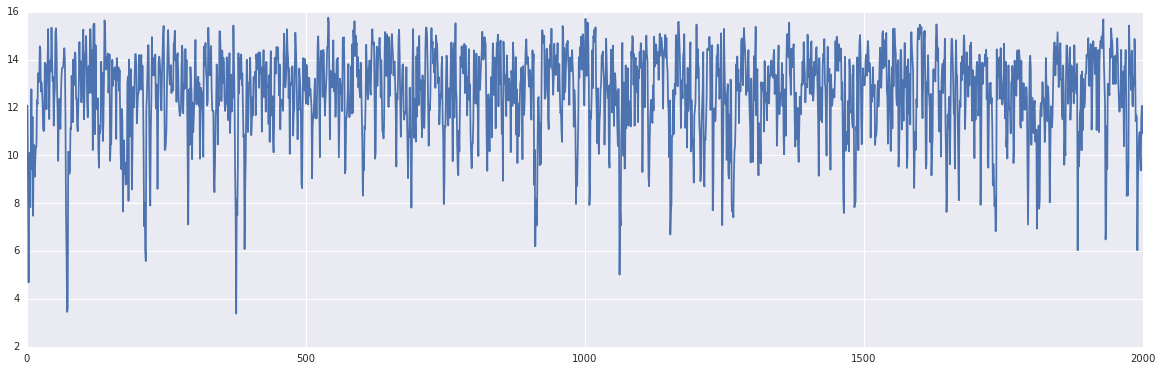
\includegraphics[scale=0.4]{stochasticprocesses}
\end{figure}

Por simplicidad de notación vamos a denotar \(\{X_t\}_{t \in \calT}\) al proceso estocástico, y a continuación mostraremos una clasificación que se puede encontrar en la literatura. El conjunto \(\calT\) es conocido como espacio de parámetros\footnote{No confundir con el concepto de parámetros de una distribución o función paramétrica.} (\emph{parameter space} en inglés), y si es un intervalo de \(\reals\) (los reales no negativos normalmente) se dice que el proceso \(\{X_t\}_{t \in \calT}\) es a tiempo continuo. Si \(\calT\) es un conjunto numerable (los números naturales normalmente), entonces se dice que el proceso \(\{X_t\}_{t \in \calT}\) es a tiempo discreto. En el caso de que \(\calT\) sea un espacio topológico de mayor dimensión (\(\reals^{d}\) por ejemplo), se dirá que \(\{X_t\}_{t \in \calT}\) es un campo aleatorio (o \emph{random field} en inglés).

La imagen de \(X_t\) es conocida como espacio de estados (o \emph{state space} en inglés). En el caso en que los estados son discretos, si el tiempo es discreto también se dice que el proceso es una cadena, y si el tiempo es continuo entonces se dice que es un proceso puntual. En cambio, si los estados y el tiempo son continuos se dice que el proceso es continuo, y si sólo el tiempo es discreto entonces se dice que el proceso es una sucesión discreta de variables aleatorias, donde una realización parcial del proceso se llama serie temporal.

\subsection{Teorema de Consistencia de Kolmogorov}

Así como existe el concepto de función de distribución para variables aleatorias, este se puede extender al caso multidimensional de forma directa. Sea \(X_1, \dotsc, X_n\) un conjunto de variables aleatorias. La función de distribución conjunta del vector aleatorio \((X_1, \dotsc, X_n)\) es de la forma
\[F(c_1, \dotsc, c_n) = \prob(\{\omega : X_i(\omega) \leq c_{i} \text{ para todo } i\}).\]

Mientras que el enfoque de teoría de la medida parte con un espacio de probabilidades para definir a los procesos estocásticos, el enfoque de aprendizaje de máquinas parte desde una colección de leyes finito-dimensionales, que mediante el Teorema de Consistencia de Kolmogorov es posible construir modelos predictivos.

\begin{definition}
	La familia de distribuciones finito-dimensionales del proceso estocástico \(\{X_t\}_{t \in \calT}\) es una colección de funciones \(\calF = \{F_{t_1, \dotsc, t_n} : t_1, \dotsc, t_n \in \calT, n \in \naturals\}\) que, dada una colección finita cualquiera de puntos \(t_1, \dotsc, t_n\in \calT\), la distribución conjunta del vector aleatorio \((X_{t_1}, \dotsc, X_{t_n})\) está dada por \(F_{t_1, \dotsc, t_n} (c_{1}, \dotsc, c_n)\).
\end{definition}

El conjunto \(\calF\) de familia de distribuciones finito-dimensionales satisface las bien conocidas condiciones de consistencia de Kolmogorov:
\begin{enumerate}
	\item \textbf{Permutación}: para cualquier \(n\)-permutación \(\pi\), conjunto de índices \(t_1, \dotsc,t_{n} \in \calT\) y valores \(x_1, \dotsc,x_n \in \calX\) se tiene que
	\[F_{t_{\pi(1)}, \dotsc, t_{\pi(n)}} \left(x_{\pi(1)}, \dotsc, x_{\pi(n)}\right) = F_{t_1, \dotsc, t_n} \left(x_1, \dotsc, x_n\right).\]
	\item \textbf{Marginalización}: para cualquier conjunto de índices \(t_1, \dotsc, t_{n+m} \in \calT\) y todo conjunto de valores \(x_1, \dotsc, x_n \in \calX\) se tiene que
	\[F_{t_1, \dotsc, t_{n+m}} (x_1, \dotsc, x_n, +\infty, \dotsc, +\infty) = F_{t_1, \dotsc, t_n} (x_1, \dotsc, x_n).\]
\end{enumerate}

Si una familia de distribuciones finito-dimensional \(\calF\) satisface las condiciones de consistencia, entonces el \emph{Teorema de Consistencia de Kolmogorov} \cite{tao2011introduction} nos permite construir un proceso estocástico \(\hat{f} = \{\hat{f}_t\}_{t \in \calT}\) tal que su familia de distribuciones finito-dimensionales \(\hat{\calF}\) coincide con \(\calF\). La implicancia de este resultado repercute en el aprendizaje de máquinas de modo que, al tener una regla para construir un conjunto de distribuciones finito-dimensionales de forma consistente, podemos calcular probabilidades posteriores de cualquier vector aleatorio \(X\) dados los datos \(E\).

Como la ley de un proceso estocástico está completamente determinada por la asociada familia de leyes finito-dimensionales (l.f.d. de ahora en adelante) \cite{ross1996stochastic}, por abuso de notación nos referiremos a su ley como \(\calF\). Ahora podemos caracterizar al proceso \(\{X_t\}_{t \in \calT}\) según las propiedades que cumple su familia de leyes finito-dimensionales. Así como una variable aleatoria tiene media y varianza, un proceso estocástico tiene una función de media y una función de covarianza, definidas a continuación.

\begin{definition}
	Dado un un proceso estocástico \(\{X_t\}_{t \in \calT}\), sus funciones de media \(\mu\) (también denotada como \(m\)) y de covarianza \(k\) se definen como
	\begin{align*}
		\mu(t)	&= \mean(X_t), \\
		k(t, s)	&= \cov(x_t, x_s) = \mean\left[(x_t - \mu(t)) (x_s - \mu(s))\right].
	\end{align*}
\end{definition}

Cabe destacar que \(k(t, t) = \cov(x_t, x_t) = \variance(x_t)\). A continuación definiremos dos propiedades interesantes sobre las l.f.d. y las funciones de media y covarianza.

\begin{definition}
	Un proceso estocástico \(\{X_t\}_{t \in \calT}\) se dice estacionario débil si \(\mu(t) = \mu\), \(k(t, t) = \sigma^2\) y para cualquier índice \(j\), \(k(t, t + j) = k(s, s + j) = \sigma_j\).
\end{definition}

\begin{definition}
	Un proceso estocástico \(\{X_t\}_{t \in \calT}\) se dice estacionario fuerte si sus l.f.d. son invariantes a la traslación temporal, es decir, para todo \(\tau \in \calT\) se tiene que \(F_{t_1, \dotsc, t_N} = F_{t_1 + \tau, \dotsc, t_N + \tau}\).
\end{definition}

El siguiente resultado caracteriza la función de covarianza en el caso que el proceso sea estacionario fuerte, en particular estacionario débil.
\begin{proposition}
	Si \(\{X_t\}_{t \in \calT}\) es estacionario fuerte, entonces es estacionario débil. En ese caso, su función de covarianza se puede escribir en función de la distancia del tiempo, es decir \(k(t, s) = k(t - s, 0) = k_\rho( t - s)\).
\end{proposition}

En general, un proceso estacionario débil no es necesariamente estacionario fuerte. Sin embargo, la clase de procesos conocidos como procesos gaussianos cumple con la propiedad de que las nociones de estacionalidad débil y fuerte coinciden. Esta es una de mucha propiedades que poseen, que son de gran utilidad para la modelación de procesos estocásticos.

\subsection{Normal Multivariada}
Como vimos anteriormente, la función gaussiana tiene una naturaleza tan especial que la hace un objeto de estudio aplicado a diferentes áreas de las matemáticas y de las ciencias en general. Veamos a continuación como se generaliza esta función a múltiples dimensiones.

\begin{figure}[h]
	\centering
	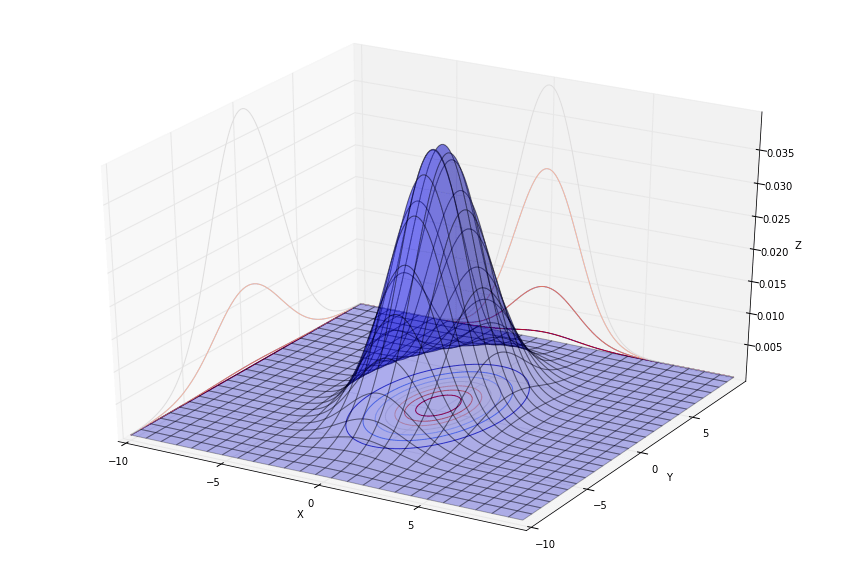
\includegraphics[scale=0.5]{gaussian2d}
\end{figure}

\begin{definition}
	Sea \(\bfx = (X_1, \dotsc, X_n)\) un vector aleatorio de dimensión \(n\). Se dice que \(\bfx\) es conjuntamente gaussiano de vector de media \(\mu_\bfx \in \reals^n\) y matriz de covarianza \(\Sigma_\bfx \in \reals^{n \times n}\) definida positiva, si su función de densidad conjunta \(f_{1, \dotsc, n}\) es de la forma
	\begin{equation*}
		f_{1, \dotsc, n}(\bfx) = \frac{1}{(2 \pi)^{\frac{n}{2}} \left\vert \Sigma_\bfx \right\vert^{\frac{1}{2}}} e^{-\frac{1}{2} (\bfx - \mu_\bfx)^\top \Sigma_\bfx^{-1} (\bfx - \mu_\bfx)}.
	\end{equation*}
\end{definition}
Por abuso de notación vamos a identificar la densidad conjunta con la distribución, es decir \(f_{1, \dotsc, n}(\bfx) = \calN_{n} (\mu_{\bfx}, \Sigma_{\bfx,\bfx})\). La siguiente proposición entrega una caracterización diferente de una normal multivariada:
\begin{proposition}
	El vector aleatorio \(\bfx = (X_1, \dotsc, X_n)\) de media \(\mu\) y matriz de covarianza \(\Sigma\) es conjuntamente gaussiana si satisface las siguientes condiciones equivalentes:
	\begin{itemize}
		\item Toda combinación lineal \(Y = a_1 X_1 + \dotsb + a_n X_n\) está normalmente distribuida.
		\item Existe una matriz \(L\) de tamaño \(n \times m\) tal que \(\Sigma = LL^\top\) y \(\bfz = (Z_1, \dotsc, Z_m)\) un vector aleatorio de \(m\) variables aleatorias normales independientes de media nula y varianza unitaria de modo que \(\bfx = L \bfz + \mu\).
	\end{itemize}
\end{proposition}
\subsection{Consistencia}

Como veremos, la distribución gaussiana satisface propiedades útiles para nuestros propósitos, es decir, las condiciones de consistencia de Kolmogorov. Sean \(\bfx : \Omega \to \calX^n, \bfxo : \Omega \to \calX^{\no}\) vectores aleatorios indexados por los tiempos disjuntos \(\bft\) y \(\bfto\) respectivamente. Si ambos vectores son conjuntamente distribuidos gaussianos entonces tenemos que
\begin{equation*}
	f_{\bft, \bfto} \left(\bfx, \bfxo\right) = \calN_{n + \no} \left( \begin{bmatrix} \mu_{\bfx} \\ \mu_{\bfxo} \end{bmatrix},
	\begin{bmatrix}
		\Sigma_{\bfx} & \Sigma_{\bfx \bfxo} \\
		\Sigma_{\bfxo \bfx} & \Sigma_{\bfxo}
	\end{bmatrix} \right).
\end{equation*}

La condición de marginalización se satisface debido a que
\[ \int_{\calX^n} f_{\bft, \bfto} (\bfx, \bfxo) \dd{\bfx} = \calN_{\no} (\mu_{\bfxo}, \Sigma_{\bfxo,\bfxo}) = f_{\bfto} (\bfxo),\]
y la condición de permutación se satisface ya que dada una \(n\)-permutación \(\pi\), existe una matriz de permutación \(P\) tal que \(P^{-1} = P^\top\) y se satisface que
\[f_{\pi(\bft)}(\pi(\bfx)) = \frac{1}{\left(2\pi\right)^{\frac{n}{2}} \left\vert P \Sigma P^\top \right\vert^{\frac{1}{2}}} e^{-\frac{1}{2} (\bfx - \mu)^\top P^\top (P\Sigma P^{\top})^{-1} P (\bfx - \mu)} = f_{\bft}(\bfx).
\]

\subsection{Procesos Gausianos}

Debido a su consistencia bajo marginalización y permutación, podemos extender la distribución gaussiana al caso infinito-dimensional gracias al Teorema de Consistencia de Kolmogorov. A esta construcción se le conoce como proceso gaussiano (o GP) \cite{rasmussen06}, que se puede interpretar como una distribución de probabilidades a priori sobre funciones que definen modelos de regresión no lineales y no paramétricos.

\begin{definition}
	Un proceso estocástico \(\{X_t\}_{t \in \calT}\) se dice un proceso gaussiano si sus distribuciones finito dimensionales son distribuciones gaussianas.
\end{definition}

Una de las principales ventajas es que un proceso gaussiano \(\{X_t\}_{t \in \calT}\) está completamente definido con su función de media \(\mu(t)\) y de covarianza \(k(t, s)\), por lo que denotamos que \(X_t \sim \GP(\mu(t), k(t, s))\). Por esta razón, la propiedad de estacionalidad fuerte coincide con la propiedad de estacionalidad débil.

\begin{proposition}
	Dado un proceso gaussiano \(\{X_t\}_{t \in \calT}\), todas sus propiedades de distribución son determinadas por sus funciones de media \(\mu(t)\) y de covarianza \(k(t, s)\). En particular, el proceso gaussiano será estacionario fuerte si su función de media es constante y la función de covarianza es en función de la diferencia temporal, es decir \(\mu(t) = \mu\) y \(k(t, s) = k_\rho(t - s)\).
\end{proposition}

\subsection{Proceso Browniano}
Uno de los procesos estocásticos más utilizado en probabilidades es el proceso de Wiener, más conocido como movimiento browniano (\emph{Brownian motion} en inglés), el cual es utilizado fuertemente para resolver ecuaciones diferenciales estocásticas y definir objetos matemáticos tales como la integral estocástica. Este proceso es un caso particular de proceso gaussiano, en donde la función de media es nula y su función de covarianza está dada por \(k(t, s) = \min\{t, s\}\).

\subsection{Machine Learning}

Los parámetros de \(\mu(t)\) y \(k(t, s)\) son llamados los \emph{hiperparámetros} del GP. En la Figura \ref{fig:gp_sunspots_example} se muestra un gráfico de un ejemplo de GP con una función de covarianza muy utilizada, llamada \emph{squared exponential} (SE), dada por
\begin{align*}
	k_{\mathrm{SE}}(t, s) = \sigma^2 \exp\left(-\frac{(t-s)^2}{l^2}\right),
\end{align*}
donde \(\sigma^2 > 0\), y \(l > 0\) son los \emph{hiperparámetros} del GP.

Dada un vector de puntos \(\bft \in \calT^n\), denotemos la evaluación de la función de media \(\mu\) en \(\bft\) de tal forma que el vector \(\mu(\bft)_i = \mu(t_i)\) para \(i \in \{1,...,n\}\). De forma análoga, dados dos vectores de puntos \(\bft \in \calT^n\) y \(\bfto \in \calT^{\no}\), denotemos la evaluación de la función de covarianza \(k\) en \(\bft,\bfto\) de modo que la matriz \([k(\bft,\bfto)]_{i,j} = k(t_i,\bar{t}_j)\) para \(i \in \{1,...,n\}\) y \(j \in \{1,...,\no\}\).

Mientras no haya ambigüedad en la selección de los puntos \(\bft\), denotaremos \(X_\bft\) como \(\bfx\), \(\mu(\bft)\) como \(\mu_{\bfx}\) y \(k(\bft,\bft)\) como \(\Sigma_{\bfx}\). Para una segunda colección de puntos \(\bfto\) la notación es análoga: la evaluación del proceso es \(X_{\bfto} = \bfxo\), la media es \(\mu(\bfto) = \mu_{\bfxo}\), la covarianza \(k(\bfto,\bfto) = \Sigma_{\bfxo}\) y la covarianza cruzada entre \(\bfx\) y \(\bfxo\) se denota \(k(\bft, \bfto) = \Sigma_{\bfx \bfxo}\).

Para hacer inferencia en nuevos \emph{inputs} \(\bfto\) basta con calcular la distribución posterior de \(\bfxo\) dada las observaciones \(\bfx\), la cual también es gaussiana y sigue la distribución
\[f_{\bfto \mid \bft}(\bfxo \mid \bfx) = \calN(\bfxo \mid \mu_{\bfxo \mid \bfx}, \Sigma_{\bfxo \mid \bfx}),\]
donde
\begin{align*}
	\mu_{\bfxo \mid \bfx}	&= \mu_{\bfxo} + \Sigma_{\bfxo\bfx} \Sigma_{\bfx\bfx}^{-1} (\bfx - \mu_{\bfx}),\\
	\Sigma_{\bfxo \mid \bfx}	&= \Sigma_{\bfxo \bfxo} - \Sigma_{\bfxo \bfx} \Sigma_{\bfx \bfx}^{-1} \Sigma_{\bfx \bfxo},
\end{align*}
se conocen como la media y la covarianza condicional respectivamente; esos estadísticos permiten calcular estimaciones puntuales, intervalos de confianza y muestrear funciones directamente. En la Figura \ref{fig:gp_sunspots_example} mostramos la posterior de un GP con kernel SE sin entrenar y con entrenar, dado un conjunto de observaciones de datos de actividad solar.

\begin{figure}[h]
	\centering
	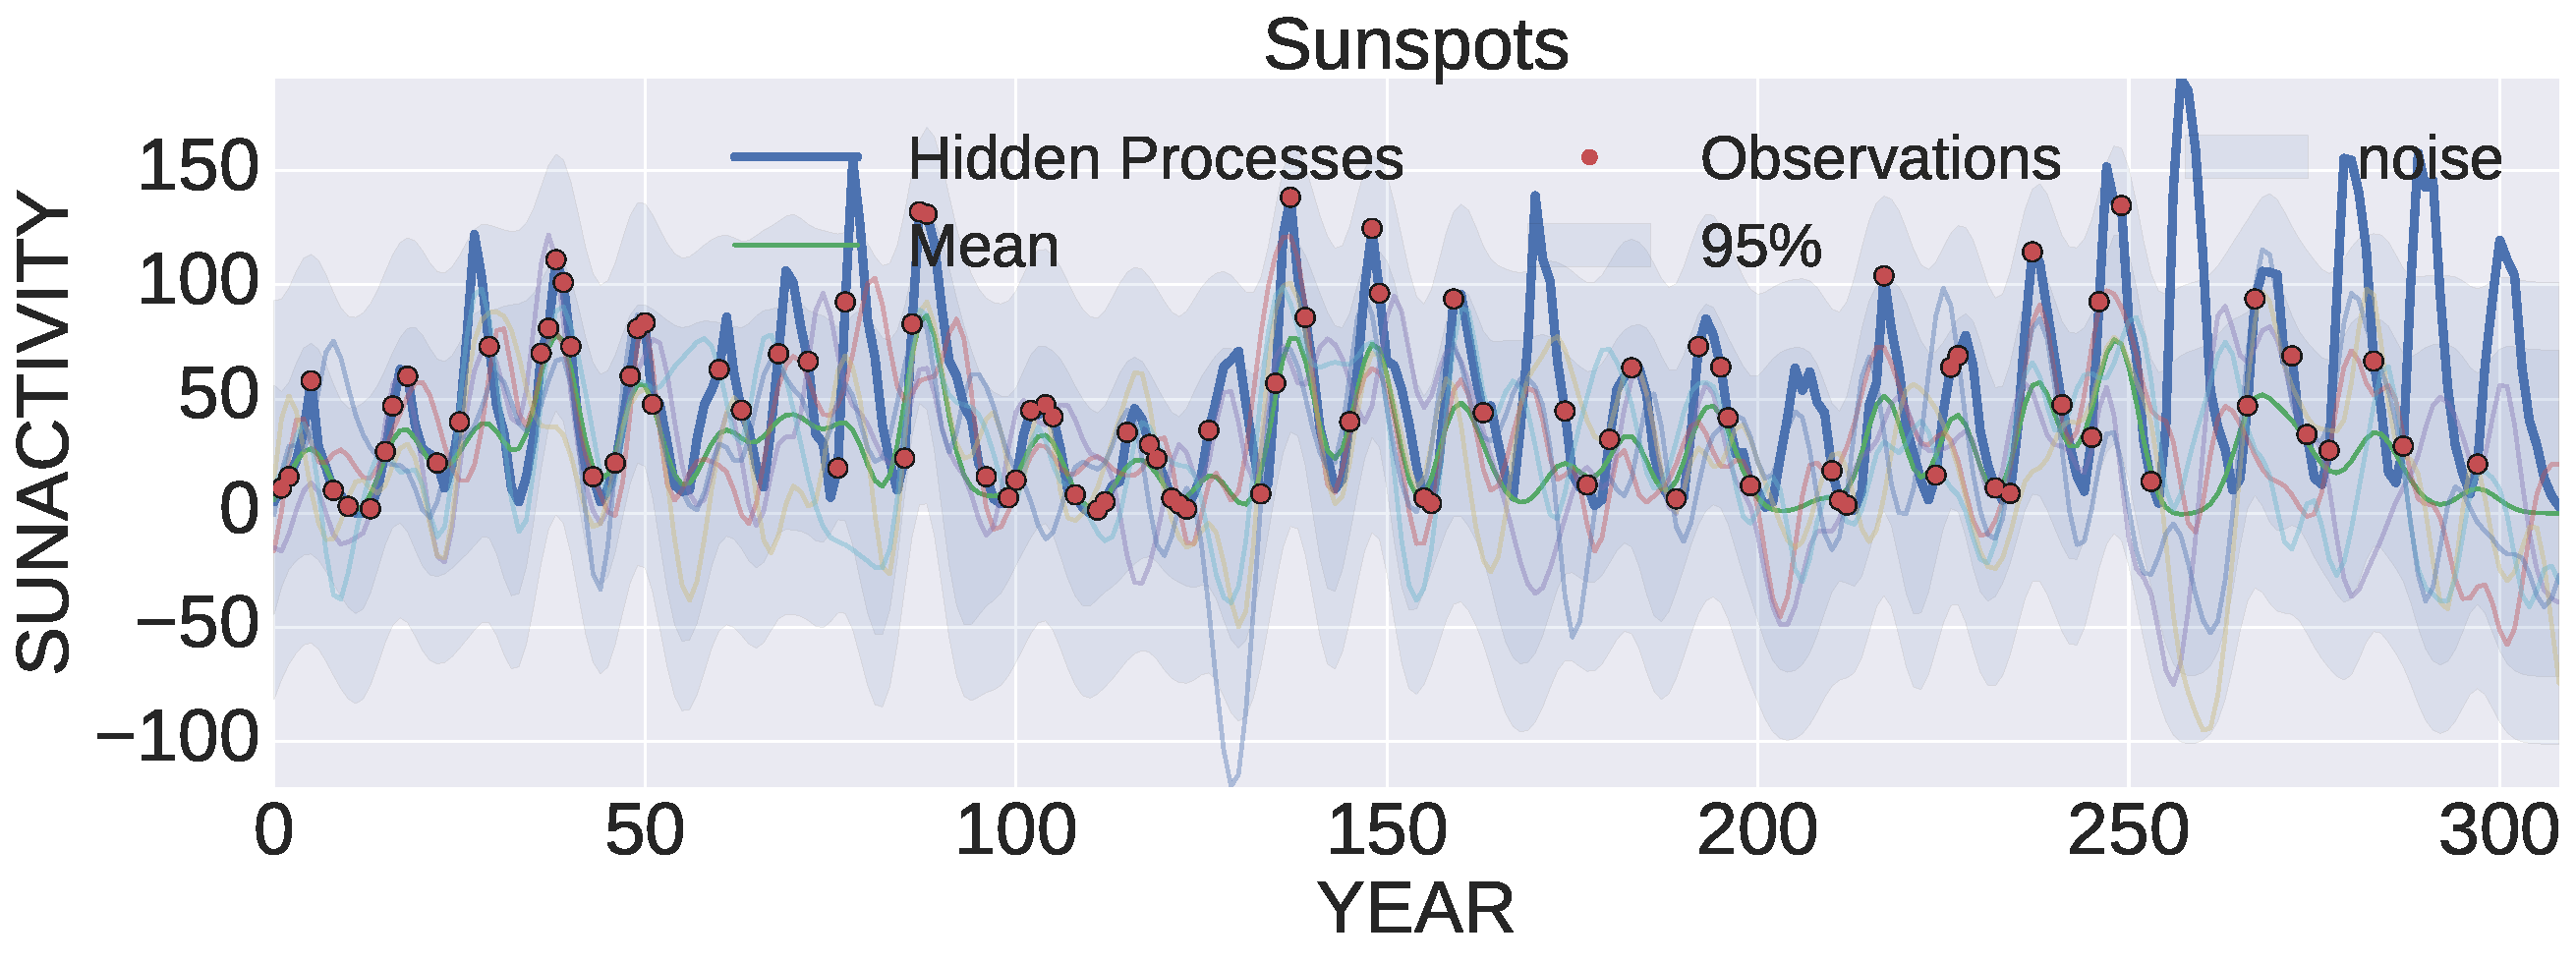
\includegraphics[width=0.49\textwidth]{gp_sunspots1}
	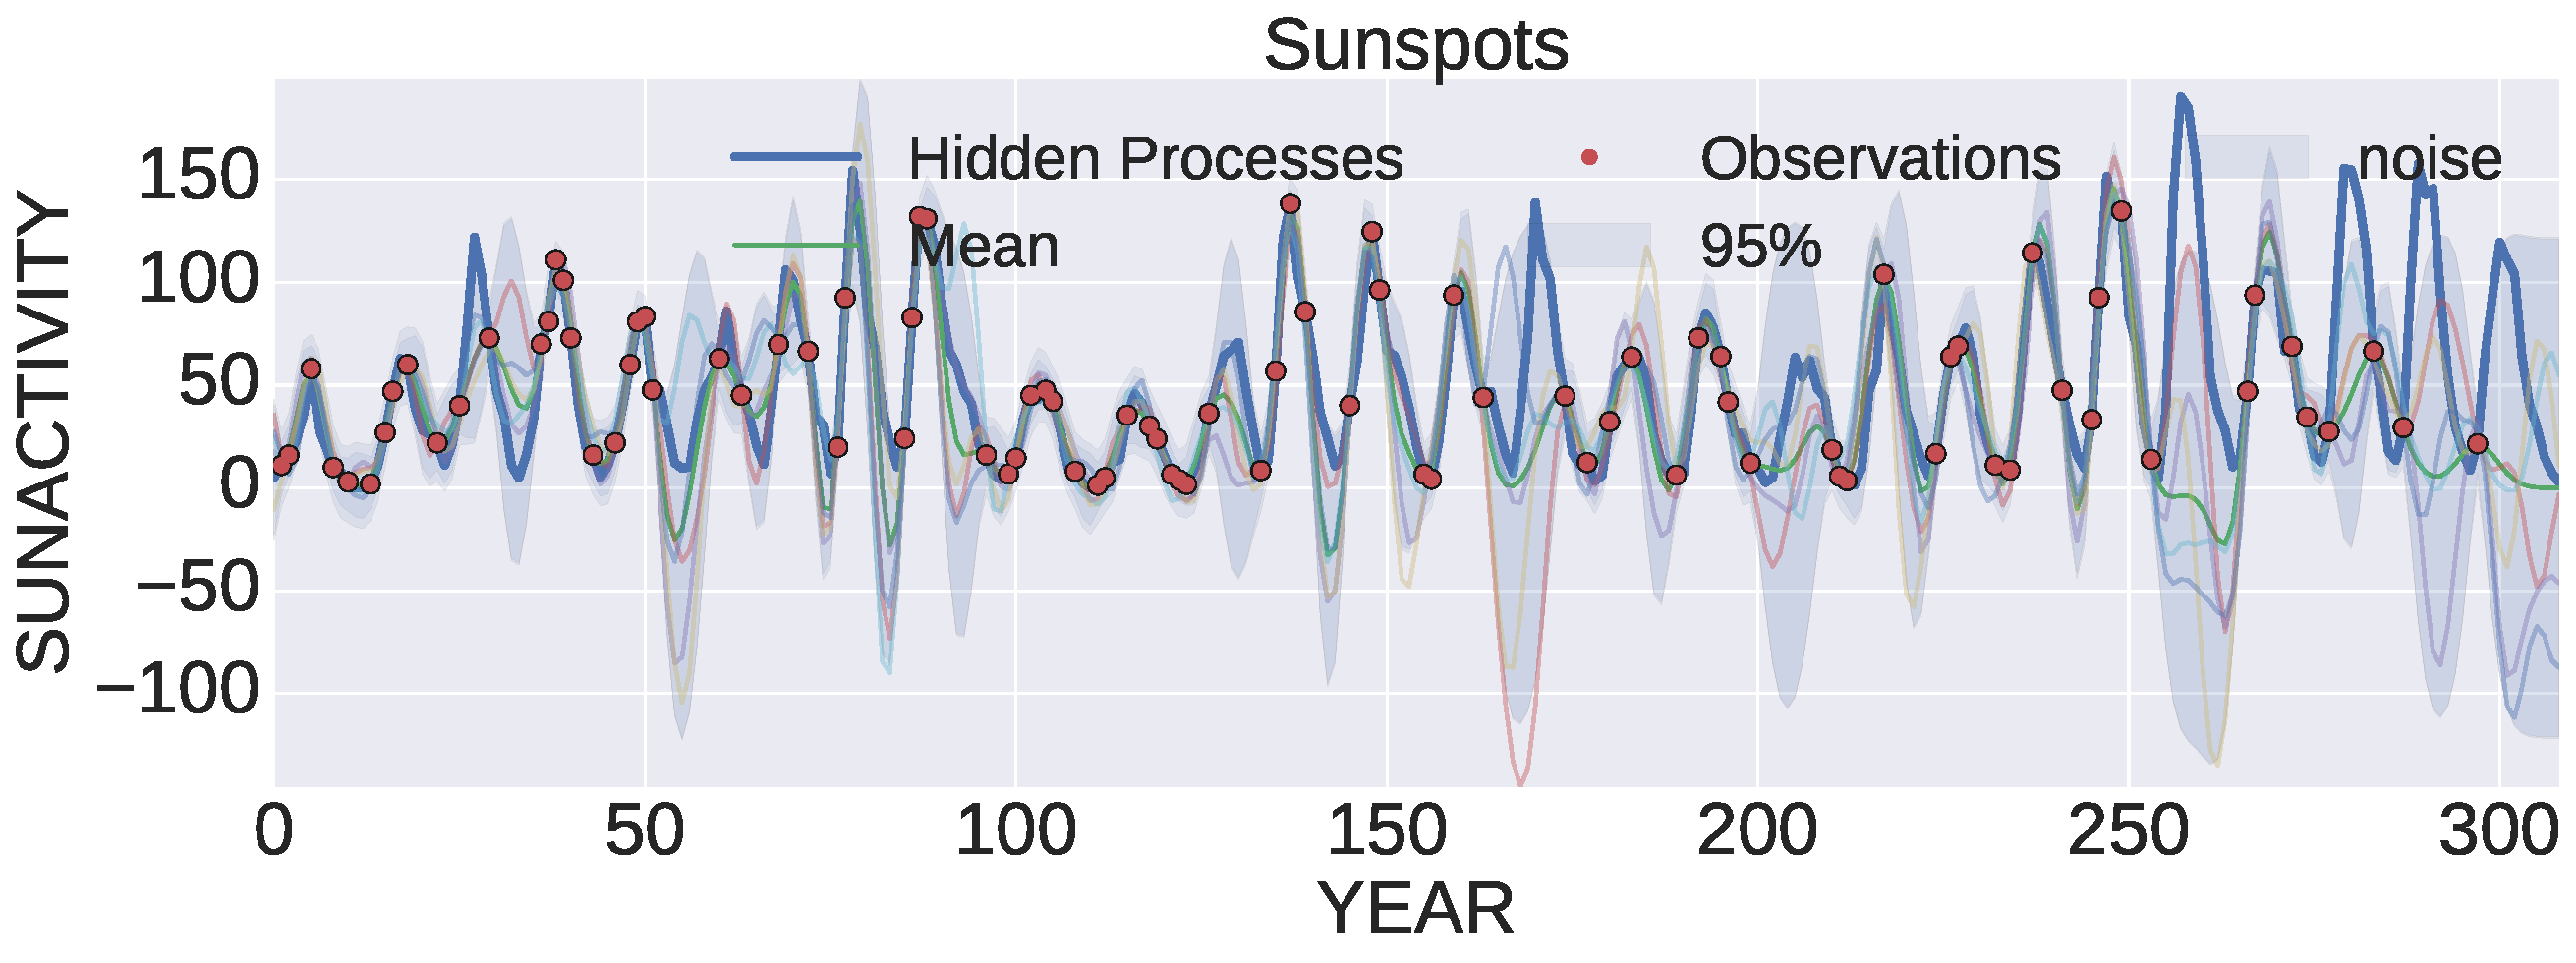
\includegraphics[width=0.49\textwidth]{gp_sunspots2}
	\caption{La distribución posterior de un GP. Izquierda: GP no entrenado. Derecha: GP entrenado.}
	\label{fig:gp_sunspots_example}
\end{figure}

El kernel usualmente se escoge heurísticamente basado en la experiencia y el conocimiento a priori del fenómeno a modelar. En la Figura \ref{fig:gp_kernels} consideramos la inferencia sobre las mismas cuatro observaciones, pero tres diferentes kernels:
\begin{itemize}
	\item Ornstein-Uhlenbeck: \(k_{\mathrm{OU}}(t, s) = \sigma^2 \exp\left(-\frac{\lvert t-s \rvert}{2l^2}\right)\),
	\item \emph{Rational Quadratic}: \(k_{\mathrm{RQ}}(t, s) = \sigma^2 \left(1 + \frac{\lvert t - s \rvert^2}{2\alpha l^2}\right)^{-\alpha}\),
	\item \emph{Locally Periodic}: \(k_{\mathrm{per}}(t, s) = \sigma^2 \exp\left(-\frac{\lvert t - s \rvert^2}{2l^2}\right) \exp\left(-\frac{2\sen^2 (\pi \lvert t - s \rvert/p)}{l^2}\right)\).
\end{itemize}
\begin{figure}[h]
	\centering
	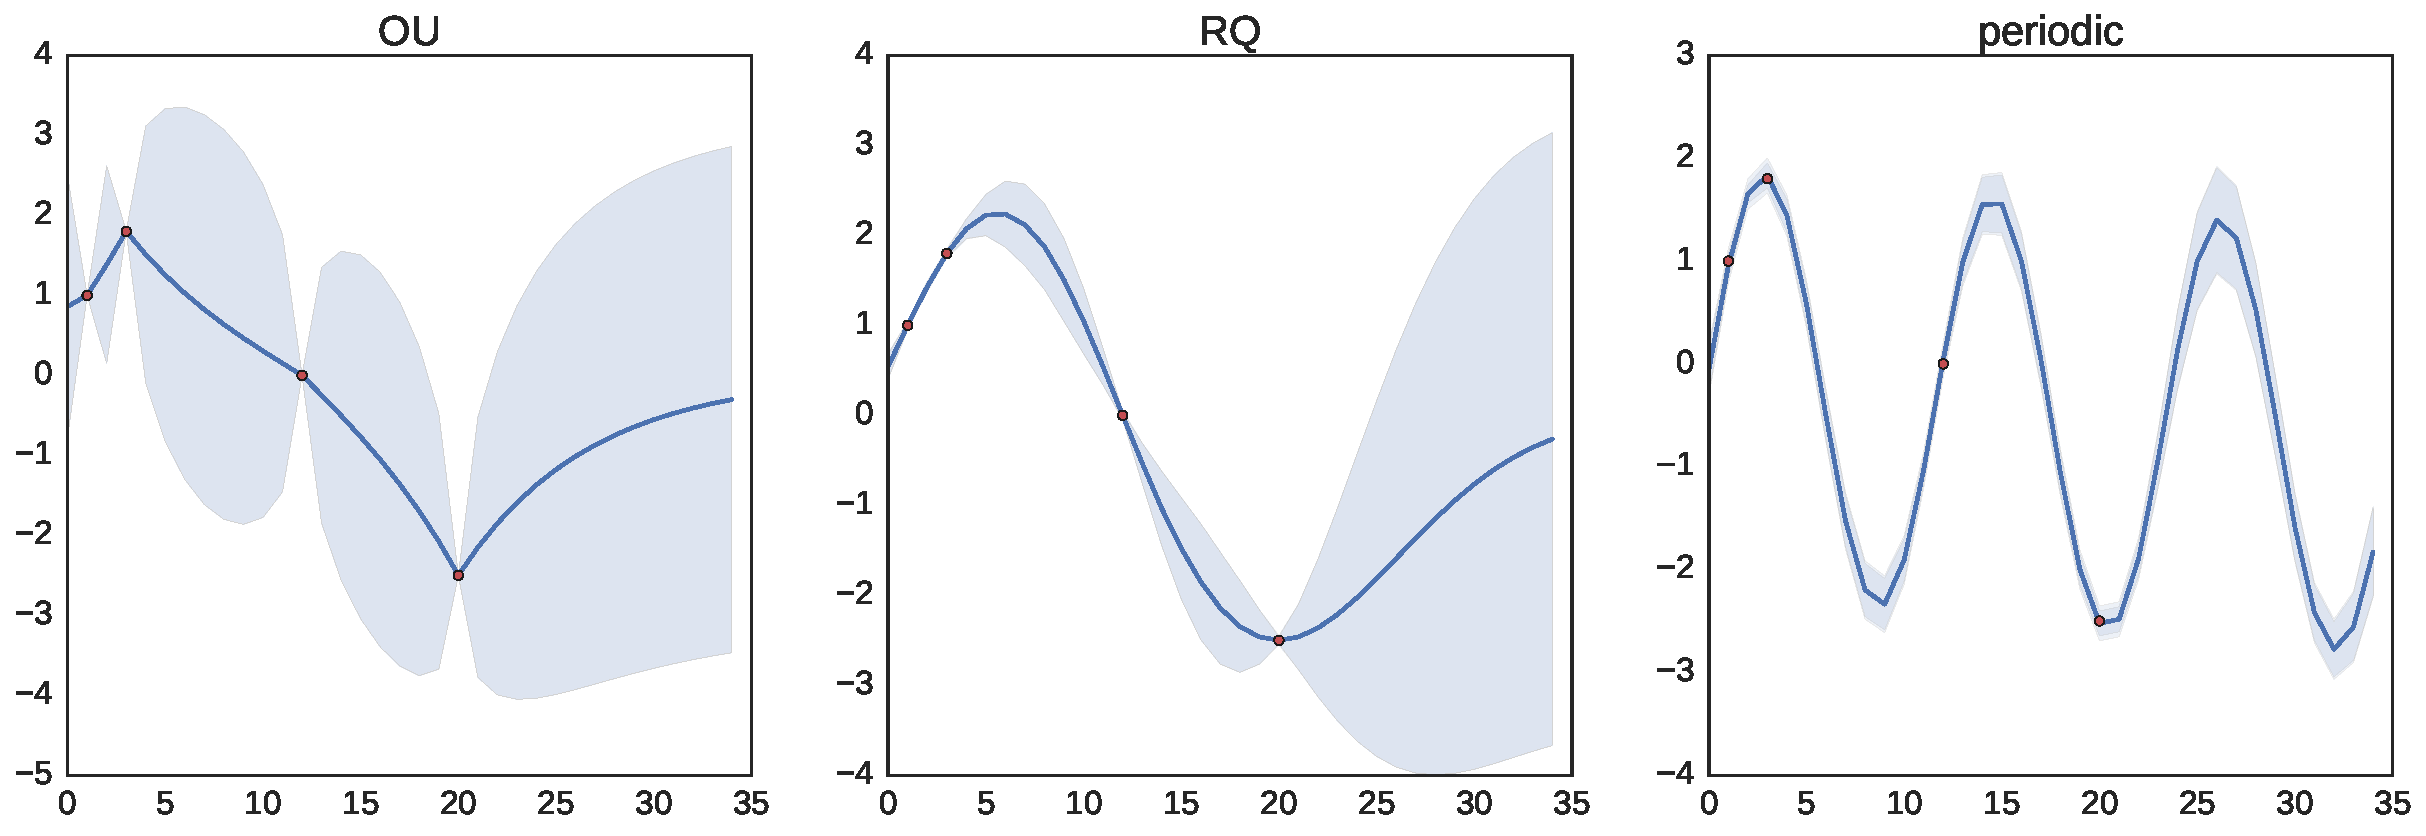
\includegraphics[width=0.8\textwidth,height=0.22\textwidth]{kernels2}
	\caption{La distribución posterior de GP con diferentes funciones de kernels, pero las mismas observaciones. Izquierda: Ornstein-Uhlenbeck, centro: \emph{Rational Quadratic}, derecha: \emph{Locally Periodic}.}
	\label{fig:gp_kernels}
\end{figure}

Dadas las observaciones \((\bft,\bfx)\), entrenar es equivalente a encontrar un kernel \(k\) y una función de media \(m\), usualmente parametrizadas por un vector de hiperparámetros finito \(\theta = (\theta_k, \theta_m) \in \reals^p\), el cual se encuentra al minimizar la log-verosimilitud negativa (NLL por sus siglas en inglés), dada por
\[-\log p_{\bft}(\bfx \mid \theta) = \frac{n}{2} \log(2\pi) + \frac{1}{2} (\bfx - \mu_{\bfx} )^\top \Sigma_{\bfx \bfx}^{-1} (\bfx - \mu_{\bfx}) + \frac{1}{2} \log \lvert \Sigma_{\bfx \bfx} \rvert,\]
donde \(\mu_\bfx\) y \(\Sigma_{\bfx \bfx}\) son la media y la covarianza de \(\bfx\) dados los hiperparámetros \(\theta = (\theta_k, \theta_m)\). Los métodos más utilizados son los basados en el gradiente de cuasi-Newton BFGS y el método libre de derivadas de Powell. En la Figura \ref{fig:gp_sunspots_example} mostramos un GP con kernel SE, dadas observaciones de datos de actividad solar, donde el gráfico de la izquierda tiene hiperparámetros por defecto, mientras que el gráfico de la derecha tiene hiperparámetros entrenados. En el caso entrenado la media pasa cerca de la señal real y los intervalos de confianza son pequeños, por lo que la predicción tiene menos incertidumbre.

\comment{Parrafo: consolidar y resumir las ideas explicadas en el capitulo, mencionar que temas se profundizarán en otras partes del libro.}

En el capítulo de procesos gaussianos vamos a volver a revisar todo esto pero con mayor detalles, pero esta sección es una rápida introducción de como utilizar este objeto matemático para hacer predicciones.